\documentclass{beamer}
\usetheme{Madrid}

\usepackage{amsmath}
\usepackage{amsfonts}
\usepackage{amssymb}
\usepackage{amsthm}
\usepackage{subcaption}
\usepackage{svg}
\usepackage{csquotes}
\usepackage{babel}
\usepackage[noabbrev, capitalise]{cleveref}

\makeatletter
%\setbeameroption{show notes on second screen}
\setbeamertemplate{navigation symbols}{}
\setbeamertemplate{page number in head/foot}{}
\setbeamertemplate{title in head/foot}{}
\setbeamertemplate{author in head/foot}{}
\setbeamertemplate{footline}
{%
  \leavevmode%
  \hbox{%
  \begin{beamercolorbox}[wd=1\paperwidth,ht=2.25ex,dp=1ex,center]{author in head/foot}%
  \end{beamercolorbox}%
}%
  \vskip0pt%
}
\makeatother

\newenvironment{conjecture}{theorem}{Conjecture}

\author{Eric Luu}
\title{Graph Structure Theory and Book Embeddings}

\begin{document}

\frame{\titlepage}

\begin{frame}
    \frametitle{Graphs}

    \begin{columns}
      \begin{column}{0.5\textwidth}
        \begin{itemize}
          \item Graph $G = (V(G), E(G))$
          \item Planar graph: embedded on plane
          \item Euler's formula: V - E + F = 2
        \end{itemize}
      \end{column}

      \begin{column}{0.5 \textwidth}
        \begin{figure}
          \centering
          \includesvg[width = 0.8\linewidth]{figures/facetriangulation.svg}
        \end{figure}
      \end{column}
    \end{columns}
\end{frame}

\begin{frame}
    \frametitle{Surfaces}
    \begin{columns}
    \begin{column}{0.5\textwidth}
      \begin{itemize}
        \item Surface = 2D manifold
        \item 2 kinds: \begin{itemize}
          \item Orientable
          \item Nonorientable
        \end{itemize}
        \item Genus = 2*handles + crosscaps
      \end{itemize}
    \end{column}
    \begin{column}{0.5 \textwidth}
      \begin{figure}
        \centering
        \includesvg[width = 0.8\linewidth]{figures/surfaces.svg}
      \end{figure}
    \end{column}
    \end{columns}
\end{frame}

\begin{frame}
  \frametitle{Books}
  \begin{columns}
    \begin{column}{0.5\textwidth}
      \begin{itemize}
        \item Book: half-planes glued on boundary
        \item Half Planes: Pages
        \item Book-embedding: Graph on book
        \begin{itemize}
          \item Vertices on boundary
          \item Edges on pages
          \item No edges cross
        \end{itemize}
        \item Pagenumber: Least number of pages to embed a graph.
      \end{itemize}
    \end{column}
    \begin{column}{0.5\textwidth}
        \begin{figure}
          \centering
          \includesvg[width = 0.8\linewidth]{figures/3page_K5.svg}
        \end{figure}
    \end{column}
  \end{columns}
  \note{Books were introduced by Persinger + Atneosen in the 1960s
  Book-embeddings were introduced by Kainen and Ollman in the 1970s. 
  }
\end{frame}


\begin{frame}
  \frametitle{Planar Book-Embeddings}
  \begin{columns}
    \begin{column}{0.5\textwidth}
        \begin{itemize}
          \item Planar Graphs can be embedded on four pages.
          \item Proven by Yannakakis
          \item Cannot be improved
        \end{itemize}    
    \end{column}
      \begin{column}{0.5\textwidth}
        \begin{figure}
          \centering
          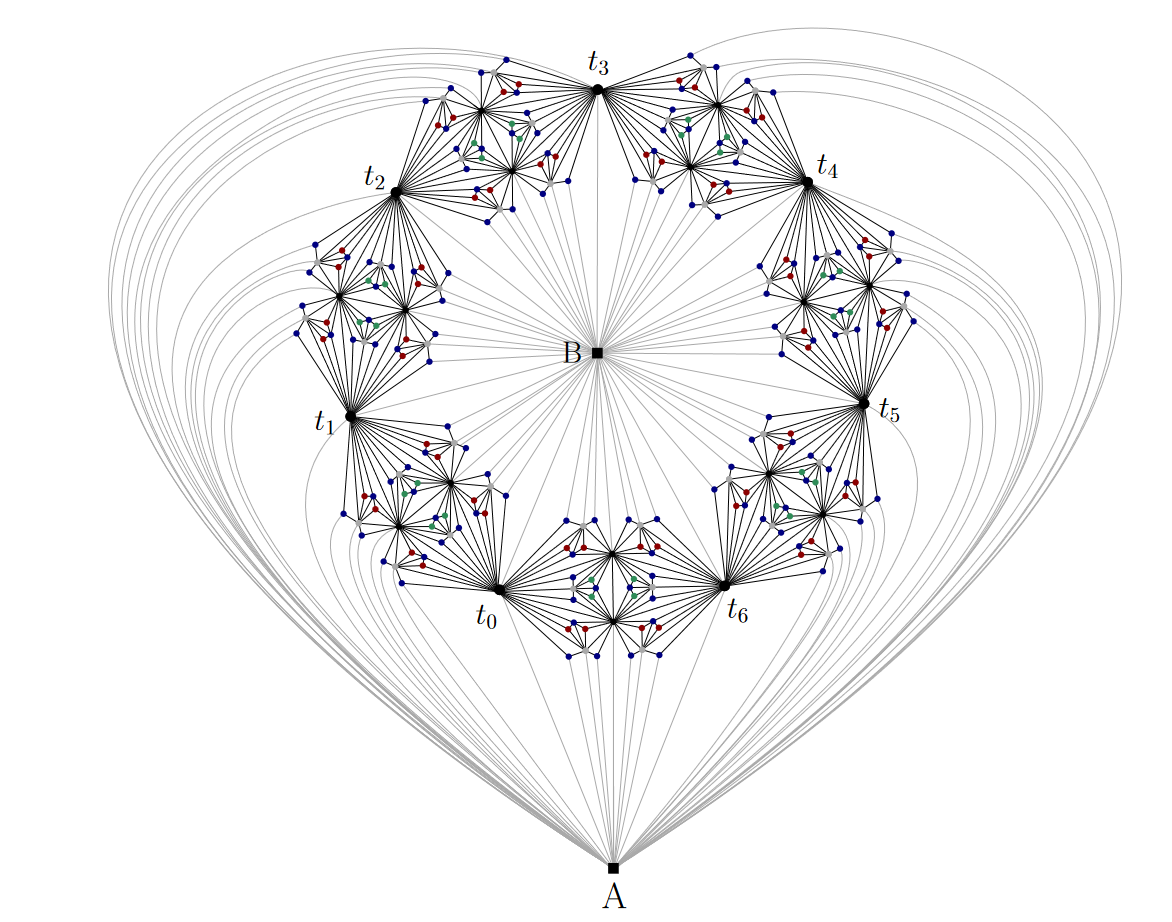
\includegraphics[width = \linewidth]{figures/Screenshot 2024-09-26 152422.png}
        \end{figure}
    \end{column}
  \end{columns}
  \note{
    Originally thought to be unbounded
    Simple algorithm embeds on nine pages by Buss and Shor
    Improved to 6 by Heath
    Yannakakis improved to 4
    Claimed to have unpublished proof for four decades
    Proven by Yannakakis in 2020, other paper with authors Bekos, Kaufmann, Klute, Pupyrev, Raftopoulou, Uedkerdt also proved this in 2020.
  }
\end{frame}

\begin{frame}
    \frametitle{Minors}
    \begin{columns}
      \begin{column}{0.5\textwidth}
          \begin{itemize}
            \item $H$ is \textbf{minor} of $G$ if $H$ obtained from $G$ through \begin{itemize}
              \item vertex deletion
              \item edge deletion
              \item edge contraction
            \end{itemize}
            \item $G$ is $H$-minor-free if $H$ is not a minor of $G$. 
          \end{itemize}    
      \end{column}
        \begin{column}{0.5\textwidth}
          \begin{figure}
            \centering
            \includesvg[width = \linewidth]{figures/edge_contraction.svg}
          \end{figure}
      \end{column}
    \end{columns}
\end{frame}

\begin{frame}
	\frametitle{Main Conjecture}
		\begin{conjecture}
		Every $K_t$-minor free graph is embeddable on $f(t)$ pages.
	\end{conjecture}
	
	\begin{corollary}
		Every minor-closed family can be embedded on bounded number of pages.
	\end{corollary}
	\note{Minor-closed family is family closed under taking minors
		Examples of minor-closed families: planar graphs, Graphs embedded on surfaces etc}
\end{frame}

\begin{frame}
    \frametitle{Graph Minor Structure Theorem}
    \begin{itemize}
      \item $K_t$ minors can be built up from 4 ingredients
    \end{itemize}
\end{frame}

\begin{frame}
  \frametitle{Ingredients}
\end{frame}

\begin{frame}
  \frametitle{Open Problems}
\end{frame}


\end{document}